% include a brief discussion about how the limitation of leaf instances affects the performance of the decision tree algorithm.

\documentclass[11pt,a4paper,twocolumn]{article}
% \usepackage{times} % times font
% \usepackage{mathptmx} % times font in maths
\usepackage[top=0.5in, bottom=0.7in, left=0.5in, right=0.5in]{geometry}
\usepackage{multirow} %in tables
\usepackage{caption} % in tables
\usepackage{lipsum}
\pagenumbering{gobble}
\newcommand{\HRule}{\rule{\linewidth}{0.5mm}}
\usepackage[pdftex]{graphicx}

% \usepackage{fullpage}
% \usepackage{amsmath}
% \usepackage{hyperref}
% \usepackage{graphicx}
% \usepackage{subfigure}
% \usepackage{indentfirst} % indent frst paragraph of section
% \usepackage[usenames,dvipsnames]{color}
% \newcommand{\ts}{\textsuperscript}

\begin{document}

\twocolumn[
\begin{@twocolumnfalse}
\begin{center}
	\begin{large}
	{\HRule \\[0.2cm]}
	\textsc{Assignment 2: Object Recognition--- Task 1}
	{\HRule \\[0.3cm]}
	\end{large}

{	\begin{minipage}{ 0.4\textwidth }
		\begin{flushleft}
			Kacper \textbf{Sokol} --- \texttt{ks1591}\\
			Maciej \textbf{Kumorek} --- \texttt{mk0934}
		\end{flushleft}
	\end{minipage}
	\begin{minipage}{ 0.4\textwidth }
		\begin{flushleft}
			{Image Processing \&\\ Computer Vision $|$ COMS30121}
		\end{flushleft}
	\end{minipage}
}

{\begin{small}
~\\[0.1cm]
\emph{Remark:} \textbf{FD}--- face(s) detected; \textbf{TP}--- true positive; \textbf{FP}--- false positive; \textbf{FN}--- false negative
\end{small}}

\end{center}
\end{@twocolumnfalse}
]

\section*{Obama faces set}
\begin{itemize}
\item \texttt{obama0.jpg}--- 1 \textbf{FD}--- \textbf{TP}--- detection is pretty straight forward, whole face is visible--- model example of face.
\item \texttt{obama1.jpg}--- 0 \textbf{FD}--- \textbf{FN}--- the face is angled and features are not trained for rotated regions.
\item \texttt{obama2.jpg}--- 1 \textbf{FD}--- \textbf{TP}--- there was enough features available in the image such as eyes, nose, ears or hair to find a face.
\item \texttt{obama3.jpg}--- 0 \textbf{FD}--- \textbf{FN}--- the bright light reflection covered half of face what stopped classifier from matching symmetric features of face.
\item \texttt{obama4.jpg}--- 2 \textbf{FD}--- \textbf{TP}, \textbf{FP}--- enough part of face was visible to collect needed features to recognize it. The other detection is not correct because of gradual change of blue color in the sky possibly due to \textit{jpg} compression. The effect is visible in \textit{Image: ~/ref{img:false-positive}}.
\item \texttt{obama5.jpg}--- 0 \textbf{FD}--- \textbf{FN}--- left half of the face is covered with hand what prevents classifier to match certain features such as eyes.
\item \texttt{obama6.jpg}--- 4 \textbf{FD}--- \textbf{TP}, 3 \textbf{FP}--- the face is detected but 3 other objects are misclassified as faces. Shading of the hand could resemble human face. Dark square recognized as a face is similar to \texttt{obama4.jpg} case. Mouth are detected as face possibly due to black circular shadow formed in the corner of the lips which may be recognized as eyes.
\item \texttt{obama7.jpg}--- 0 \textbf{FD}--- \textbf{FN}--- the face is not detected because the photo is taken from the side-- no symmetrical features. From this point of view there is no match for eye and hair is covering greater region of head.
\item \texttt{obama8.jpg}--- 0 \textbf{FD}--- \textbf{FN}--- The face is not found because proportions of it are changed due to image being squeezed, what leads to features not being matched.
\item \texttt{obama9.jpg}--- 0 \textbf{FD}--- \textbf{FN}--- .
\item \texttt{obama10.jpg}--- 1 \textbf{FD}--- \textbf{TP} --- .
\item \texttt{obama11.jpg}--- 2 \textbf{FD}--- \textbf{TP}, \textbf{FP} --- .
\end{itemize}

\begin{figure}[htbp]
\centering
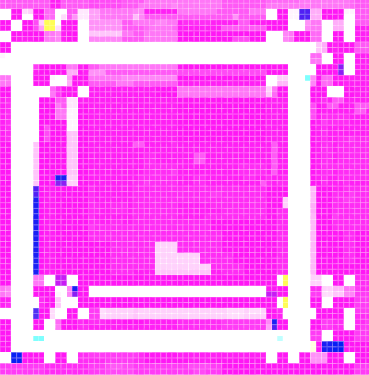
\includegraphics[width=0.1\textwidth]{false-positive.png}
\caption{False positive in \texttt{obama4.jpg}.\label{fig:false-positive}}
\end{figure}

\section*{Team faces set}
\begin{itemize}
\item \texttt{team0.jpg}--- 1 \textbf{FD}--- \textbf{TP} --- .
\item \texttt{team1.jpg}--- 2 \textbf{FD}--- \textbf{TP}, \textbf{FP} --- .
\item \texttt{team2.jpg}--- 1 \textbf{FD}--- \textbf{TP} --- .
\item \texttt{team3.jpg}--- 0 \textbf{FD}--- \textbf{FP} --- .
\item \texttt{team4.jpg}--- 1 \textbf{FD}--- \textbf{TP} --- .
\item \texttt{team5.jpg}--- 2 \textbf{FD}--- \textbf{TP}, \textbf{FP} --- .
\end{itemize}

\section*{Conclusions}
Blah blah blah.


\end{document}
